\documentclass[border=2pt]{standalone}
\usepackage{tikz}
\usetikzlibrary{arrows.meta,chains,%
                    decorations.pathreplacing}
\usetikzlibrary{matrix,positioning,arrows.meta,arrows}

\tikzset{
mymat/.style={
  matrix of nodes,
  nodes in empty cells,
  text height=1.5ex,
  text depth=0.75ex,
  text width=2.25ex,
  align=center,
  column sep=-\pgflinewidth
  }
}
\tikzset{
  rows/.style 2 args={
    sub@rows/.style={row ##1 column #2/.style={nodes={rectangle,draw=black}}},
    sub@rows/.list={#1}
  },
  box/.style 2 args={
    sub@box/.style={rows={#1}{##1}},
    sub@box/.list={#2}
  }
}
\begin{document}

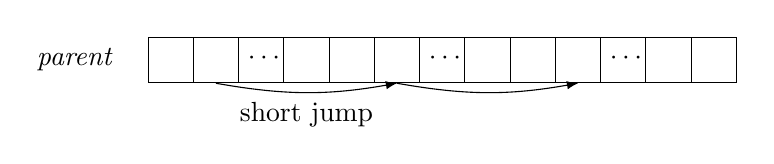
\begin{tikzpicture}[>=latex]
\matrix[mymat,anchor=west, nodes={rectangle,draw}]
at (0,0) 
(mat1)
{ 
  & & $\cdots$ & & & & $\cdots$ & & & & $\cdots$ & & \\};


\node[left=5pt of mat1]
{
   \textit{parent} \\
};

\path[solid,->](mat1-1-2.south) edge [bend right=10] node[black,midway,below=0pt] {short jump} (mat1-1-6.south);
\path[solid,->](mat1-1-6.south) edge [bend right=10] (mat1-1-10.south);

\end{tikzpicture}

\end{document}